\documentclass[letter]{article}

\usepackage[english]{babel}
\usepackage[utf8]{inputenc}
\usepackage{amsmath}
\usepackage[colorinlistoftodos]{todonotes}
\usepackage{makecell}
\usepackage{multirow}
\usepackage{caption}
\usepackage{subcaption}
\usepackage{graphicx}
\usepackage{hyperref}
\usepackage{float}
\usepackage[all]{hypcap}
\usepackage[space]{grffile}
\usepackage{enumitem}

\newlist{questions}{enumerate}{1}
\setlist[questions, 1]{label = \arabic*}
\newlist{bonus}{enumerate}{1}
\setlist[bonus, 1]{label = Bonus \arabic*}



% Adjust margins
\addtolength{\oddsidemargin}{-0.75in}
\addtolength{\evensidemargin}{-0.75in}
\addtolength{\textwidth}{1.5in}
\addtolength{\topmargin}{-.5in}
\addtolength{\textheight}{1.5in}

\title{CS 520: Assignment 2 - MineSweeper, Inference-Informed Action}
\author{Haoyang Zhang, Han Wu, Shengjie Li, Zhichao Xu}
\date{\today}

\begin{document}
\maketitle

\section{Introduction, group members and division of workload}
\label{sec:Introduction}

In this group project, we implemented a minesweeper solver that far exceeded our expectation. Not only can our program solve the normal minesweeper, but also it can solve minesweeper with inaccurate information. Our program also has a gorgeous GUI and can visualize the progress of solving minesweeper by animation. \\
\begin{tabular}{| p{2.5cm} | p{\textwidth -3.5cm} |}
	\hline
	\makecell[c]{Name \\ RUID} & Workload \\
	\hline
	\makecell[c]{Haoyang Zhang \\ 188008687} & {Implemented the minesweeper solver. Finished the writing of report for most of the questions.} \\
	\hline
	\makecell[c]{Han Wu \\ 189008460} & {Ran tests and generated figures for question \hyperref[han]{2.4}. Finished the writing of report for question \hyperref[han]{2.4}} \\
	\hline
	\makecell[c]{Shengjie Li \\ 188008047} & {Designed and implemented the GUI of our program. Implemented a function that can generate animation of the progress of solving minesweeper. Finished the format design of whole report using \LaTeX. } \\
	\hline
	\makecell[c]{Zhichao Xu \\ 188008912} & {Proofread the report. Ran tests and generated figures for question \hyperref[zhichao1]{2.5} and question \hyperref[zhichao2]{4.1}. Finished the writing of report for question \hyperref[zhichao1]{2.5}.} \\
	\hline
\end{tabular}


\section{Questions and Writeup}
\label{sec:Questions and Writeup}
\begin{enumerate}
	\item {Representation: How did you represent the board in your program, and how did you represent the information / knowledge that clue cells reveal?} \\
	\\
	In our program, the basic board is represented by a matrix, which is constructed by a 2-dimensional array. For example, a $ 64 \times 64 $ board is represented by an array of 64 elements, and each element is an array with length of 64. 
	
	The board is represented by 4 matrices:  ``covered'', ``flag'',  ``\_mine'' and ``\_clue''. 
	\begin{itemize}
		\item {The matrix ``covered'' saves exploration status. }
		\item {The matrix ``flag'' records blocks that agents regard as mines.} 
		\item {The matrix ``\_mine'' represents the distribution of mines.} 
		\item {The matrix ``\_clue'' is a preprocessed matrix that records each block’s hint number. The hint number here is used to save time when solving minesweeper.} 
	\end{itemize}   
	
	The knowledge base is represented by 9 matrices: ``covered'', ``safe'', ``flag'', ``hint'', ``warn'', ``left'', ``done'', ``nebr'' and ``prob''. 
	\begin{itemize}
		\item {Matrix ``covered'' and ``flag'' are the same as the board’s matrix.}
		\item {Matrix ``safe'' records the blocks that agents regard as safe blocks.}
		\item {Matrix ``hint'' saves the hint number the agents have got from the minesweeper.}
		\item {Matrix ``warn'' represents the number of each hint block’s un-flagged mines. \\ Namely, $ \text{warn} = \text{hint} - (\text{the number of neighbor flags}) $.}
		\item {Matrix ``left'' represents the number of each block’s inconclusive neighbors. \\ Namely, $ \text{left} = 8 - \text{(the number of neighbor flags-the number of neighbor uncovered)} - \text{(edge cost)} $.}
		\item {Matrix ``done'' records blocks whose neighbors are all conclusive. Such blocks could be ignored when agents are solving the minesweeper.}
		\item {Matrix ``nebr'' is a hash value matrix. It records the inconclusive neighbors of each block. Agents use it when trying to solve equations like ``$ A+B+C=2 $, $ A+B=1 $''.}
		\item {Matrix ``prob'' is actually a tensor. It records each block’s probability of being a mine block, given each neighbor’s data. Therefore, the size of ``prob'' is $ rows \times columns \times 9 $ (with an extra basic probability).}
	\end{itemize}         
	
	\item {Inference: When you collect a new clue, how do you model / process / compute the information you gain from it? i.e., how do you update your current state of knowledge based on that clue? Does your program deduce everything it can from a given clue before continuing? If so, how can you be sure of this, and if not, how could you consider improving it?} \\
	\\
	There are at least 3 things we need to do:
	\begin{enumerate}
		\item {Compute ``warn'' value of the block we have just explored.}
		\item {Update all neighbors’ ``left'' and ``nebr'' value.}
		\item {Update all these 9 blocks’ neighbor’s ``prob'' value.}
	\end{enumerate}
	
	If the updated "prob" value of a block is 0 or 1, it is now conclusive. Therefore, we add this block to the waiting line, to be explored or marked flag in the future.
	
	Sure that there are many other things we might make deductions, for instance, trying to combine it with a clue we have already known. However, there is a reason for stopping combining clues. Combining clues is especially time-consuming without a proper direction or heuristic. For a given knowledge base, the statements we can deduce do not change, even if we add more hints into the knowledge base. Therefore, it is not economical to spend so much time combining clues when we can explore and make deductions from somewhere else, because new hints may easily lead to exactly the same statements.
	
	If we have nothing else to do, there are still several ways to combine them (the detailed introduction is in ``$\backslash$docs$\backslash$Solution Algorithm Explanation.html''). The structure of some hints (value relationship and geometric relationship) tends to be solvable, and then we can focus on those structures. At least, we can use proof by contradiction to combine a large number of hints at one time, though it is also time-consuming.
	
	\item {Decisions: Given a current state of the board, and a state of knowledge about the board, how does your program decide which cell to search next? Are there any risks, and how do you face them?} \\
	\\
	There are mainly 4 things we can do:
	\begin{enumerate}
		\item {If there is a block in the waiting line, process it. \\ This brings no risk and is the easiest thing we can do.}
		\item {Use pattern recognition method to find a group of blocks that usually solvable, and try to solve it. \\ This performs surprisingly well, and takes not that much time, comparing with proof by contradiction.}
		\item {Use constraint satisfaction and proof by contradiction to find a conclusive block. \\ Pattern recognition could miss complex solvable structures, and therefore, we use the former one to improve. But generally, it takes too much time. Also, it has limitations. For example, it chooses some blocks randomly to search rather than choose all inconclusive blocks. Note that this limitation also leads to the missing of some solvable blocks.}
		\item {Should all attempts above fail, find a block that is worthy to take the risk to open. \\ The block should be either with the lowest risk, or ``well-paid''. A ``well-paid'' block is a block whose clue is expected to play an important role in the solving process in the future if the block itself is not a mine.}
	\end{enumerate}
	
	\label{han}
	\item {Performance: For a reasonably-sized board and a reasonable number of mines, include a play-by-play progression to completion or loss. Are there any points where your program makes a decision that you don’t agree with? Are there any points where your program made a decision that surprised you? Why was your program able to make that decision?} \\
	\\
	When we check the play-by-play progression of the game, we can find some interesting phenomena. The algorithm made many decisions to solve the problem. Some of them are consistent with human beings’ decisions, while some of them are not and surprised me (I am a human being). Let’s take a $ 10 \times 10 $ board as an example.
	
	\begin{figure}[H]
		\centering
		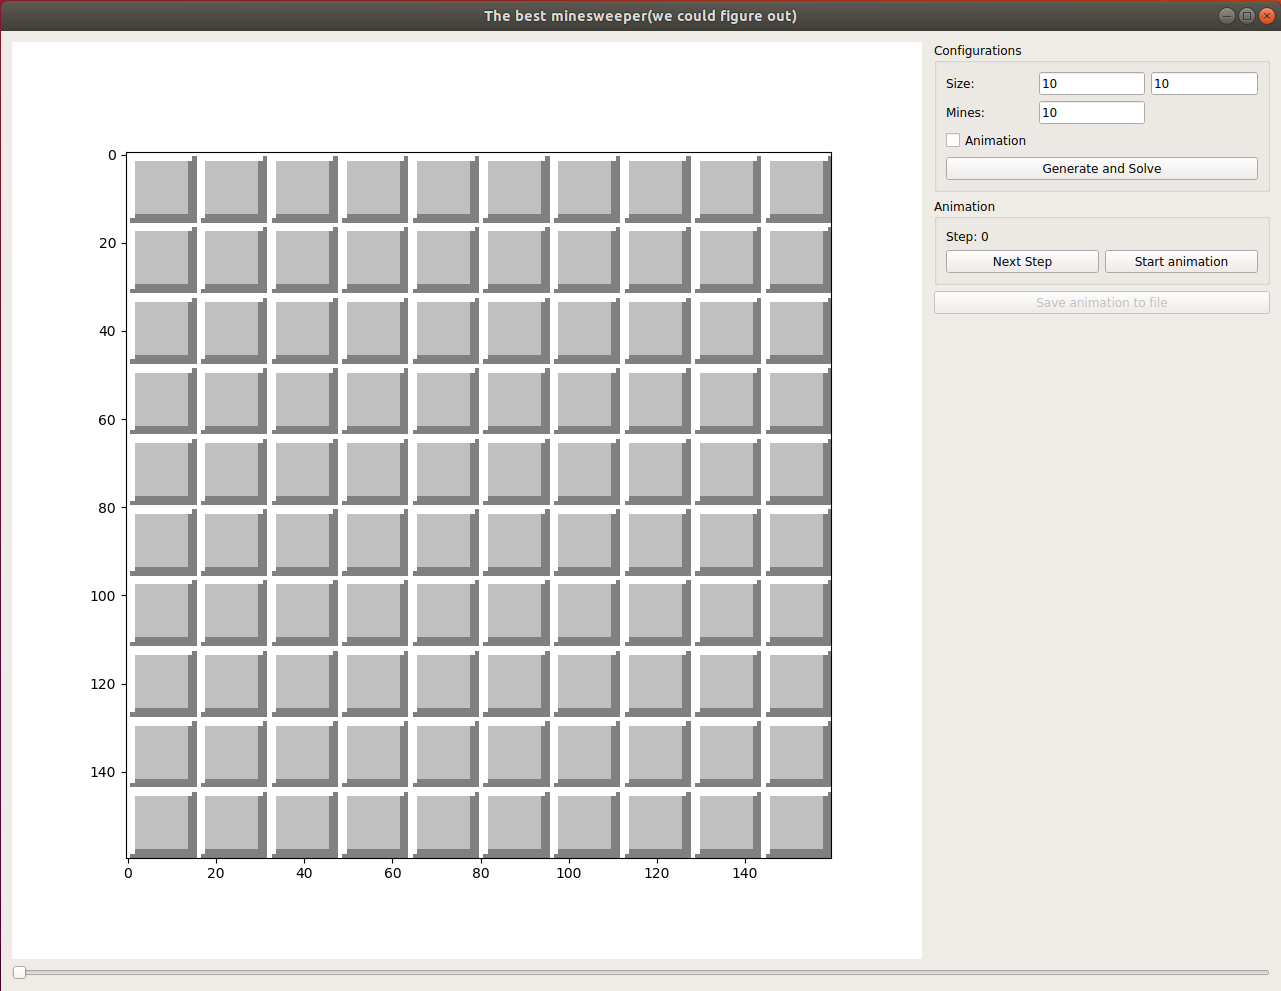
\includegraphics[width=0.75\textwidth]{../pics/1.png}
		\caption{\label{fig:1} A $ 10 \times 10 $ board.}
	\end{figure}
	As Figure \ref{fig:1} shown, it is a 10 by 10 board. There are 100 cells on the board. We use (i, j) to represent the cell in the board. ``i'' represents the row of the cell and ``j'' represents the column of the cell. For example, (1, 1) represents the cell in the upper left corner and (10, 1) represents the cell in the lower left corner. The coordinate of the cell which is uncovered in this figure is (10, 6).
	
	The first decision which the algorithm surprises me is step 13. The state of step 12 is shown below as Figure \ref{fig:2}.
	
	\begin{figure}[H]
		\centering
		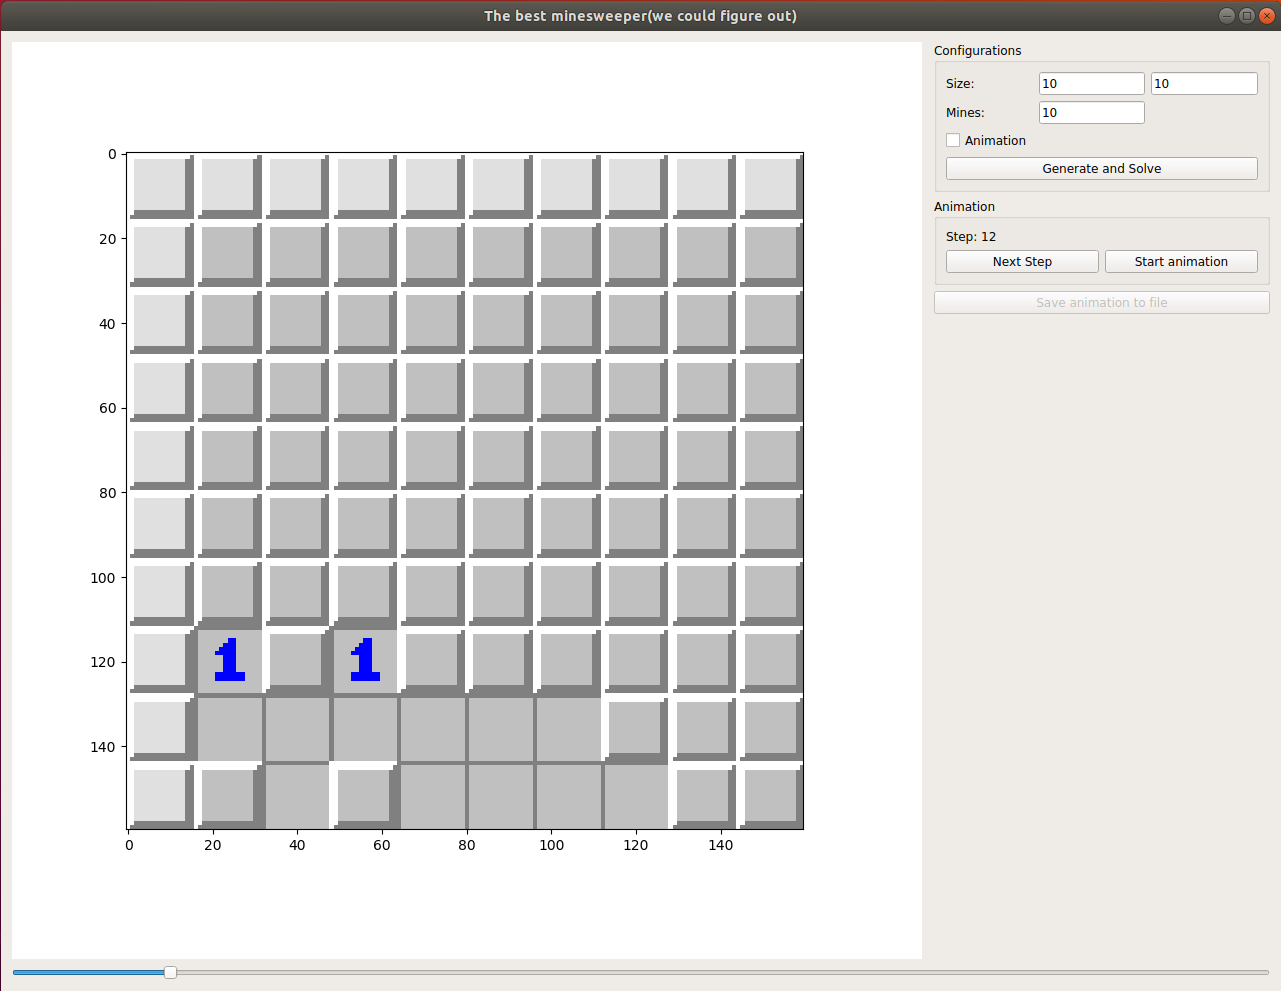
\includegraphics[width=0.75\textwidth]{../pics/2.png}
		\caption{\label{fig:2} Step 12.}
	\end{figure}
	There are already two ``1'' on the board. As a human being, I choose to explore the cells near two ``1'', because exploring more cells there can help me find the position of mine and mark it. However, the algorithm chose to check (10, 9) in the next step, which is shown in the figure below as Figure \ref{fig:3}.
	
	\begin{figure}[H]
	\centering
	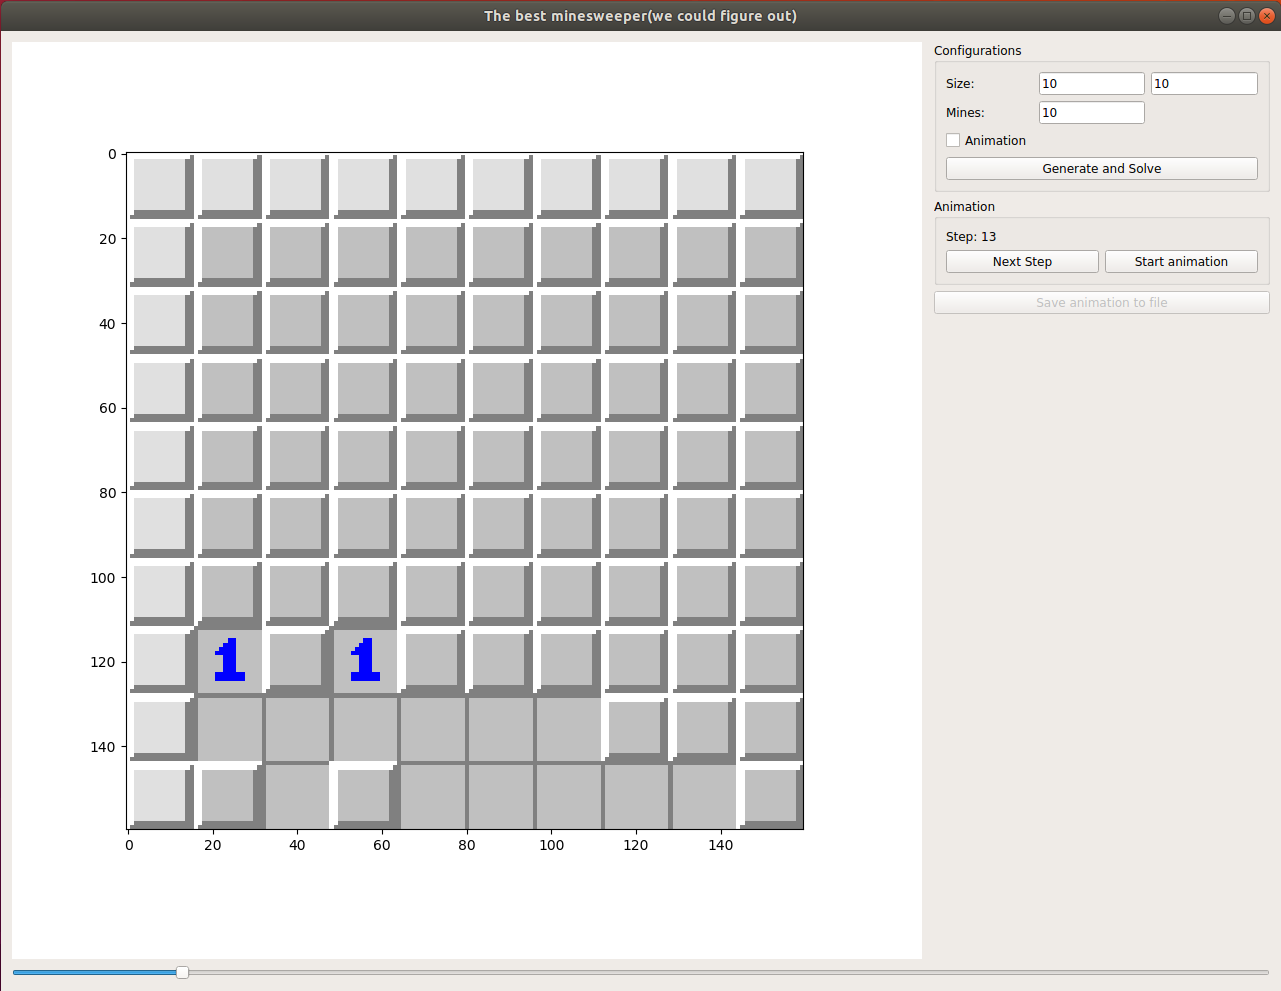
\includegraphics[width=0.75\textwidth]{../pics/3.png}
	\caption{\label{fig:3} Step 13.}
	\end{figure}
	Cell (10, 9) is far away from the two ``1'' on the board. It is safe because no number is shown on (10, 8), but it provides no help to find the mine near two ``1''. In fact, the algorithm chose to uncover (10, 4) in step 14. The choice is not a bad choice but the algorithm doesn’t know about focusing on problems, which is different from human beings and surprises me.
	
	Another thing that surprises me is in step 16 and 17.
	
	\begin{figure}[H]
		\centering
		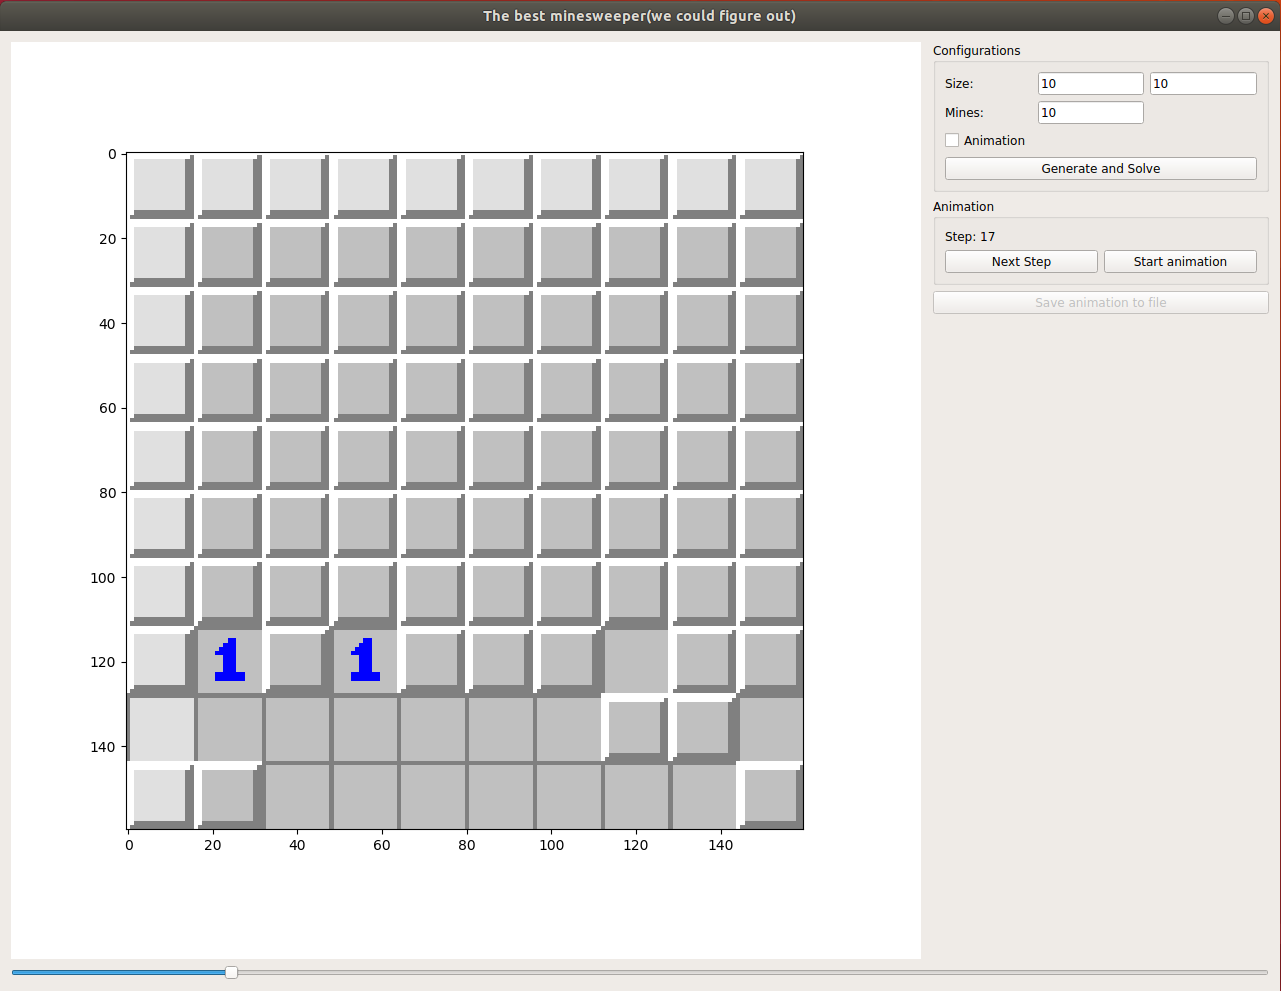
\includegraphics[width=0.75\textwidth]{../pics/4.png}
		\caption{\label{fig:4} Step 17.}
	\end{figure}
	The algorithm uncovered (8, 8) in step 16 and (9, 10) in step 17. Because of (9, 7) and (10, 9), we know that these two cells are safe. However, these two cells are not close to each other. I, as a human being, will not do like that. Human beings often uncover the neighbors of one cell and then continue to uncover the neighbors of the neighbors if they know they are safe. The randomness of this algorithm surprises me.
	
	
	Sometimes, the algorithm also made some decisions that I do not agree with. In step 42, the algorithm uncovered the cell (7, 1). We can conclude that (7, 3) is a mine according to the ``1'' shown in (8, 2). I will mark (7, 3) in the next step.
	
	\begin{figure}[H]
		\centering
		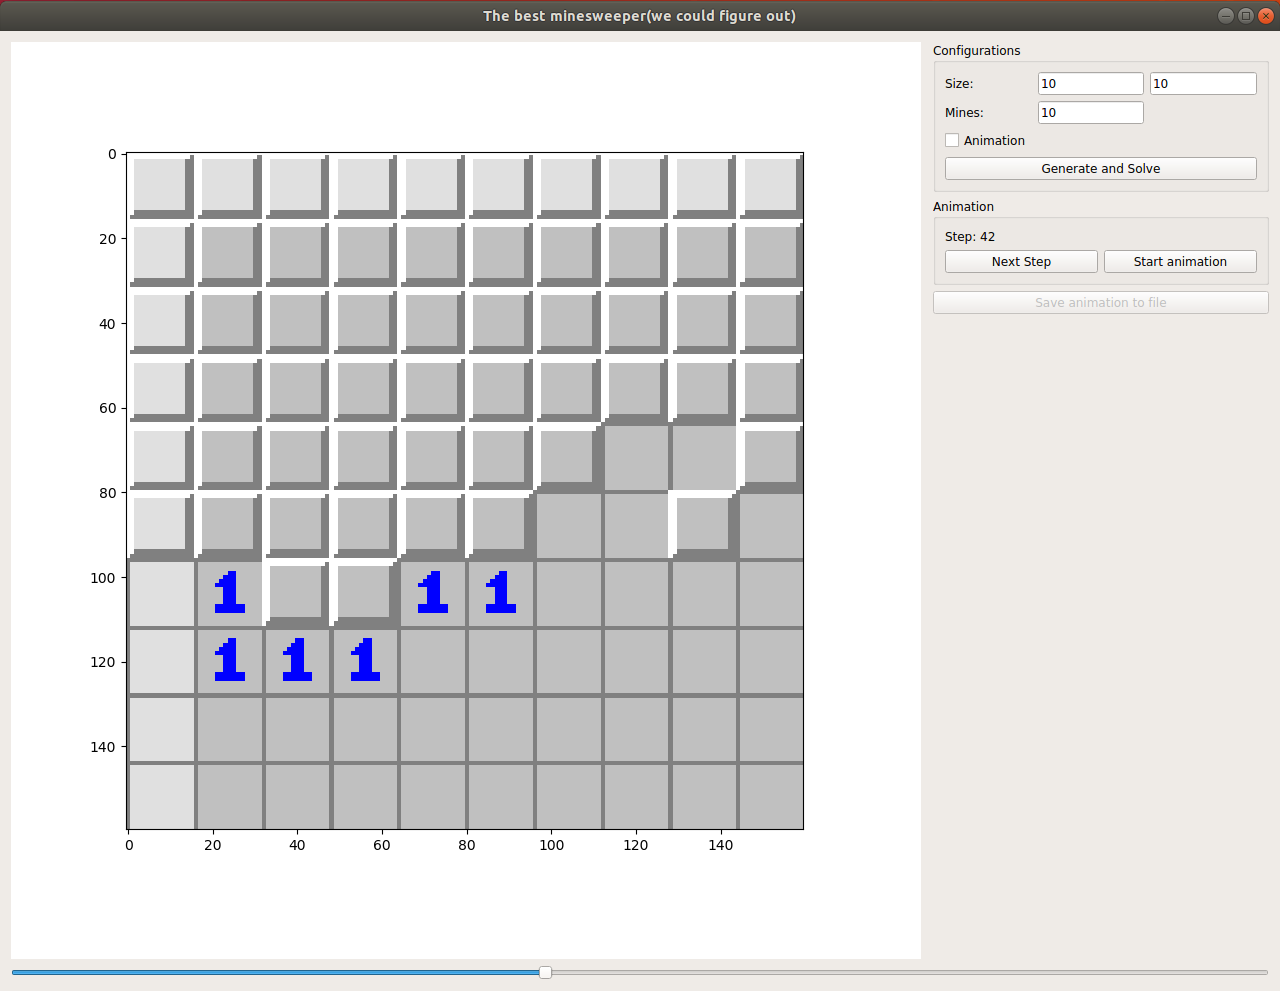
\includegraphics[width=0.75\textwidth]{../pics/5.png}
		\caption{\label{fig:5} Step 42.}
	\end{figure}
	However, the algorithm explored (4, 10) in the next step. It didn’t mark (7, 3) as mine until step 64.
	
	\begin{figure}[H]
		\centering
		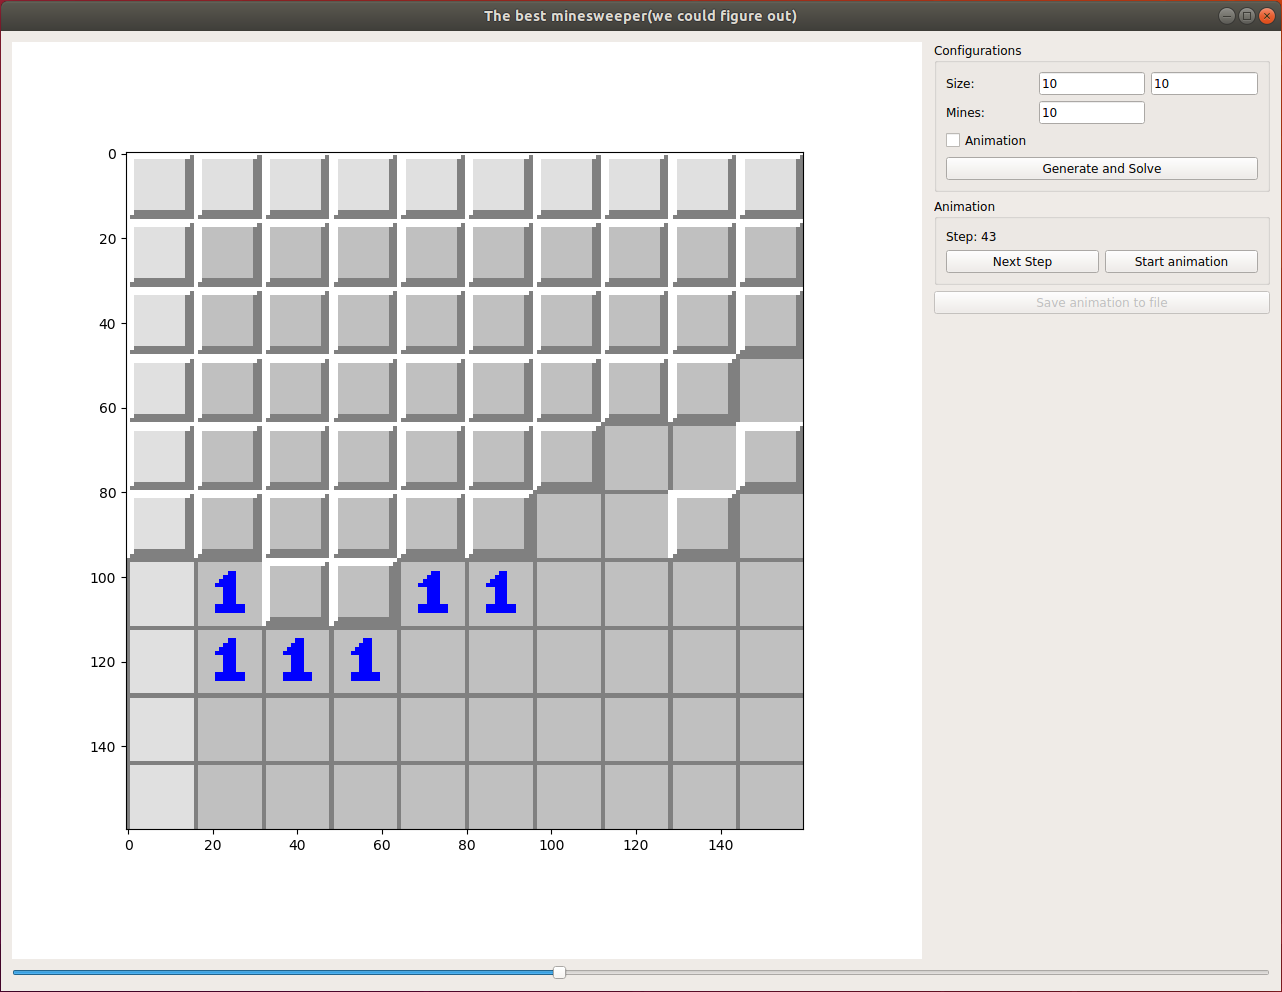
\includegraphics[width=0.75\textwidth]{../pics/6.png}
		\caption{\label{fig:6} Step 43.}
	\end{figure}
	
	The same situation happened between step 50 and step 51. In step 50, we can find that (6, 5) is a mine. However, the algorithm chose to check (3, 10) in step 51. The phenomenon is shown in Figure \ref{fig:7} and Figure \ref{fig:8}.
	
	\begin{figure}[H]
		\minipage{0.49\textwidth}
		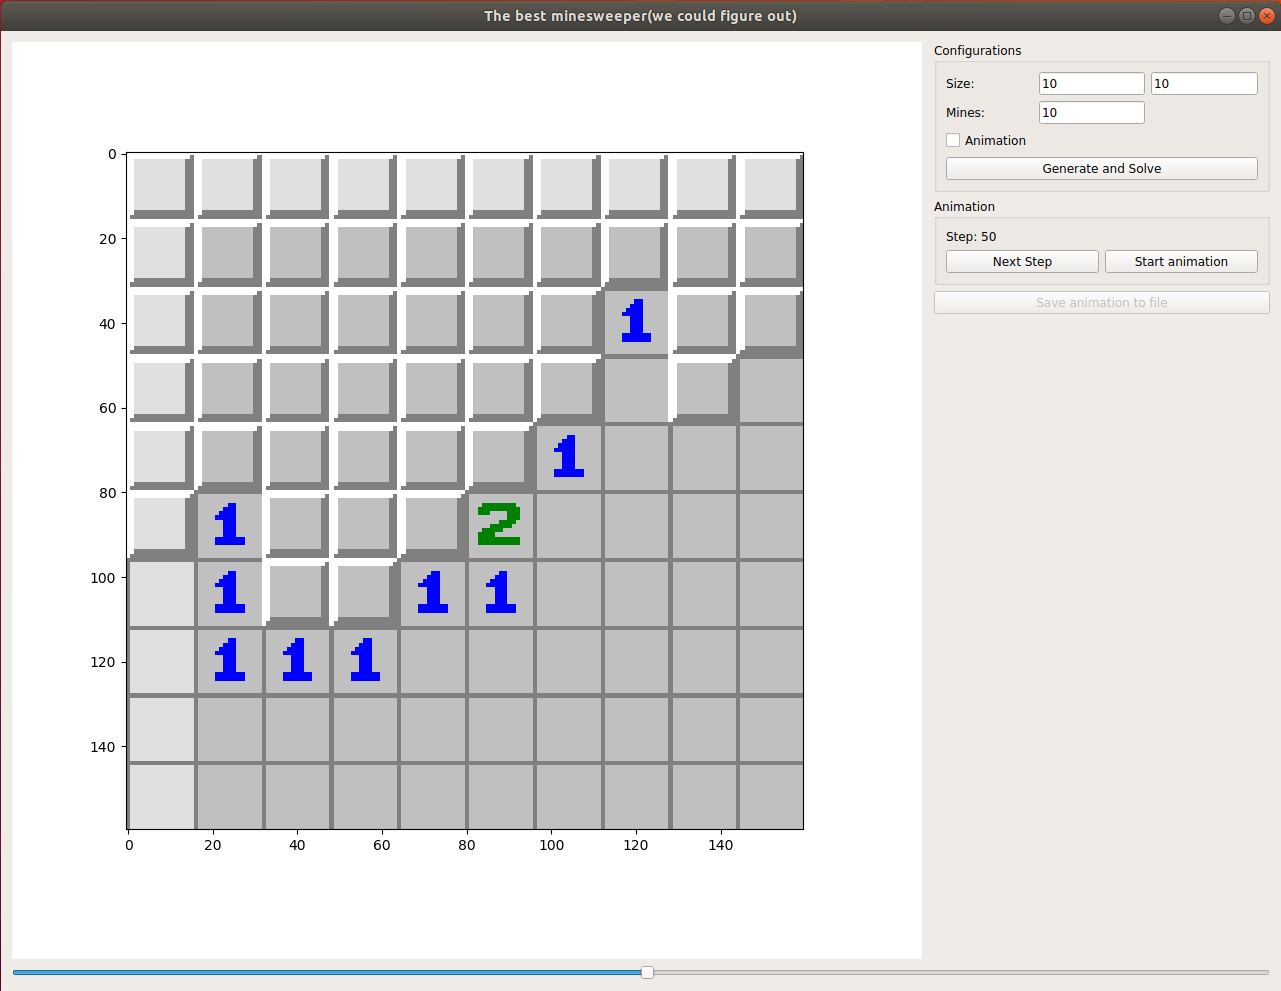
\includegraphics[width=\textwidth]{../pics/7.png}
		\caption{\label{fig:7}Step 50.}
		\endminipage\hfill
		\minipage{0.49\textwidth}
		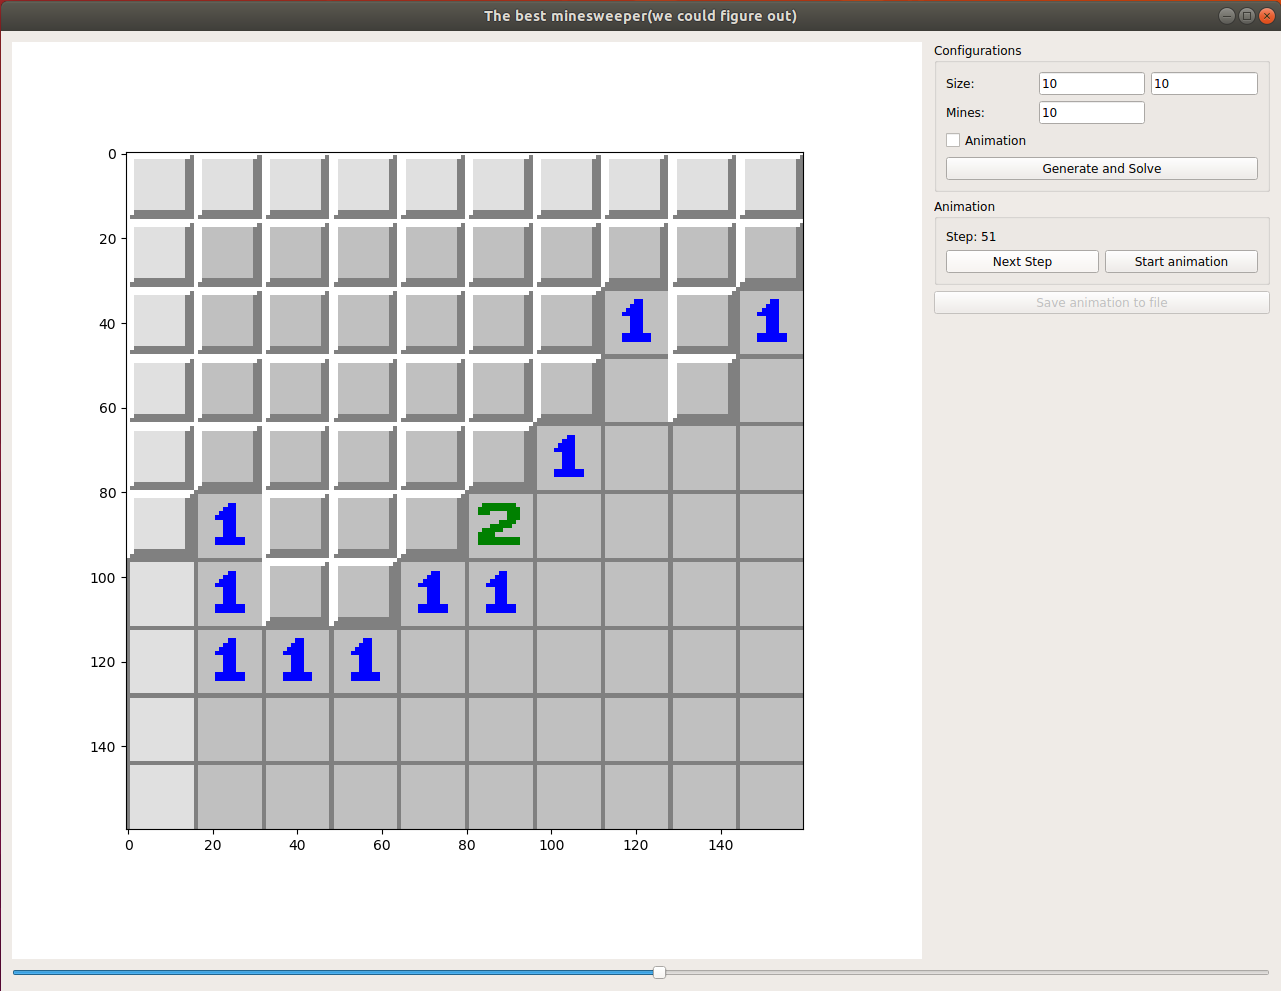
\includegraphics[width=\textwidth]{../pics/8.png}
		\caption{\label{fig:8}Step 51.}
		\endminipage
	\end{figure}
	
	In step 58, we can conclude that (6, 5) and (5, 5) are mines according to ``2'' in (6, 6). However, the algorithm chose to explore (3, 9) in step 59. The phenomenon is shown in Figure \ref{fig:9} and Figure \ref{fig:10}.
	
	\begin{figure}[H]
		\minipage{0.49\textwidth}
		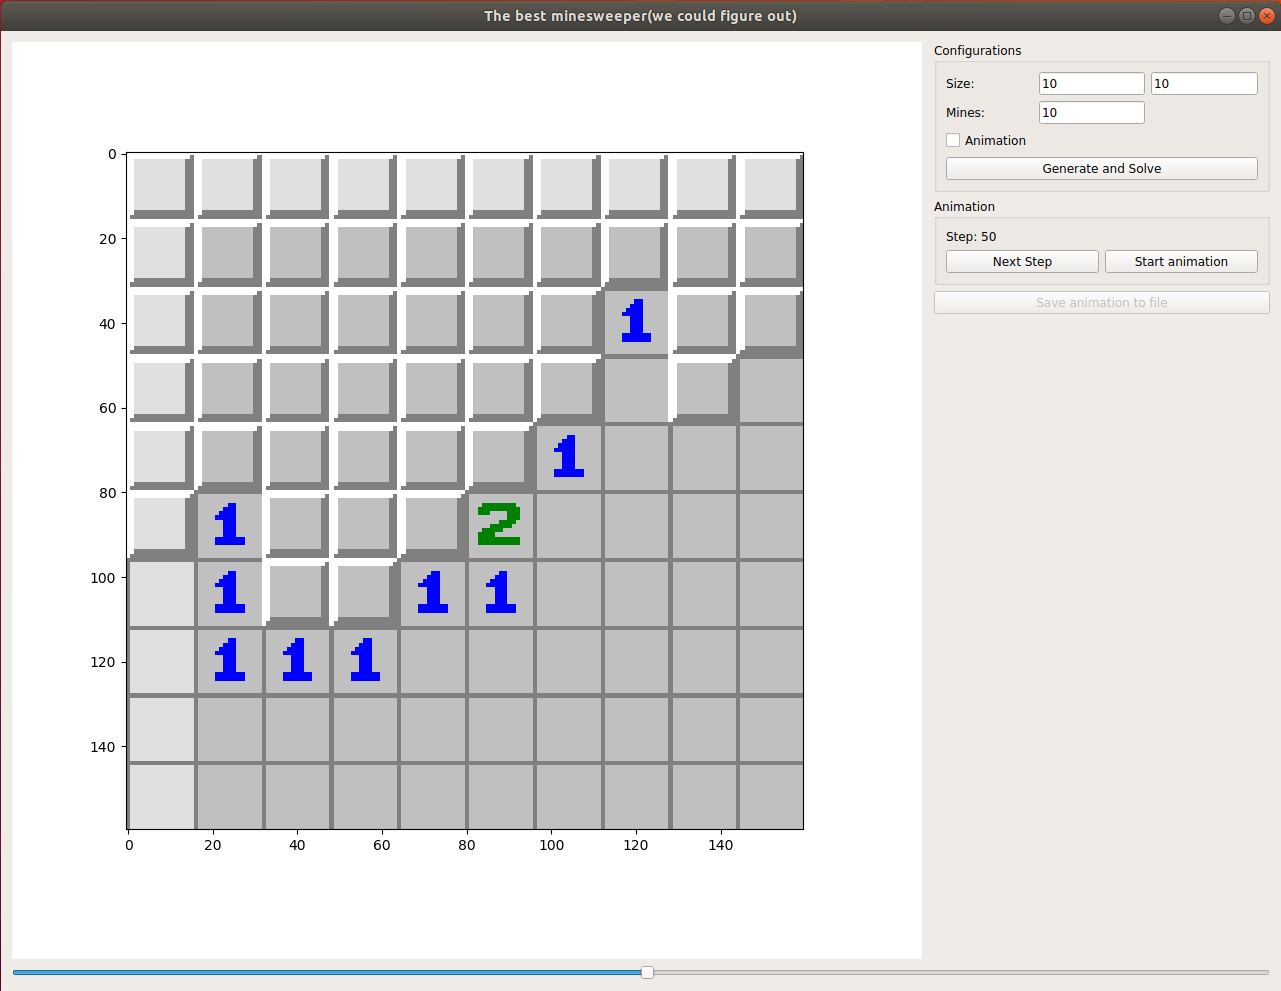
\includegraphics[width=\textwidth]{../pics/7.png}
		\caption{\label{fig:9}Step 58.}
		\endminipage\hfill
		\minipage{0.49\textwidth}
		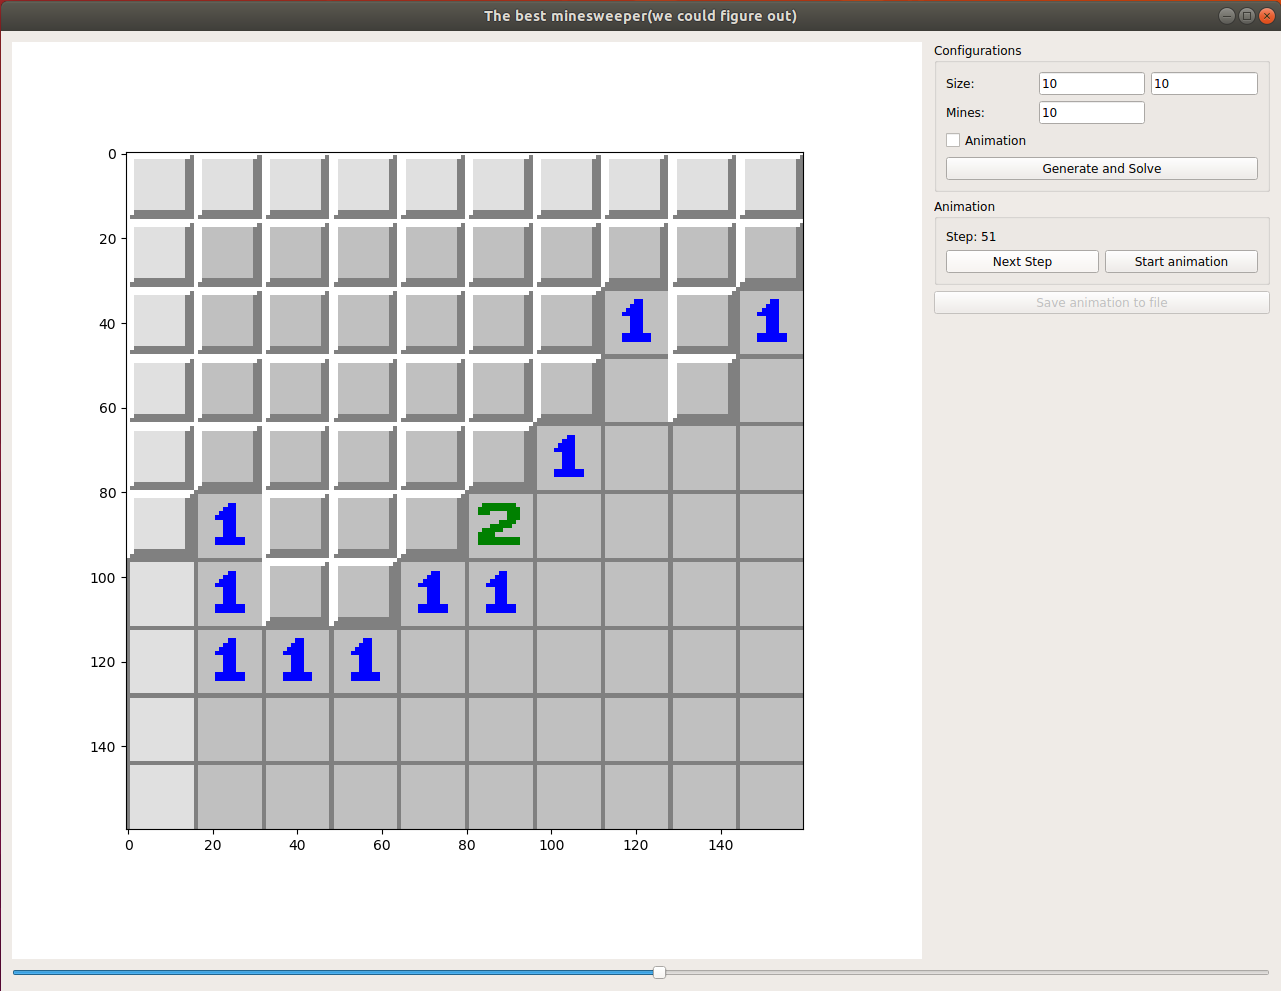
\includegraphics[width=\textwidth]{../pics/8.png}
		\caption{\label{fig:10}Step 59.}
		\endminipage
	\end{figure}
	Cell (6, 5) is marked as mine in step 63 and Cell (5, 5) is marked as mine in step 65.
	
	Sometimes, the algorithm does something that surprises me. In other times, it does something that I think is not appropriate. This is the difference between the algorithm and human beings.
	
	\label{zhichao1}
	\item {Performance: For a fixed, reasonable size of board, what is the largest number of mines that your program can still usually solve? Where does your program struggle?} \\
	\\
	We used the size of $ 64 \times 64 $ as the board size. From our preliminary testing result, our program can solve board of less than $ 20\% $ mine density easily. When the mine density is over $ 20\% $, it usually takes a much longer time. The threshold for the board to become not solvable for our program is $ 23\% $. When the mine density is over $ 23\% $, nearly all the boards are not solvable for our program. We increased the number of experiments, setting mine density to less than $ 20\% $, the result is showed in Figure \ref{fig:Mine-Density-against-Victory-Rate}.
	
	\begin{figure}[H]
		\centering
		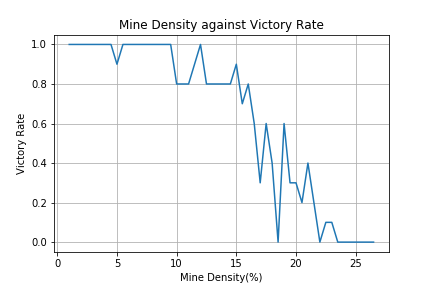
\includegraphics[scale=0.75]{../pics/Mine-Density-against-Victory-Rate.png}
		\caption{\label{fig:Mine-Density-against-Victory-Rate}Mine Density against Victory Rate.}
	\end{figure}
	
	We have come to the conclusion that our program can confidently solve boards of less than $ 20\% $ mine density. 
	As mine density increases, it takes more time to make a deduction. At the same time, there are more unsolvable scenarios where we have to take risks to explore new blocks. That’s where our program begins to struggle.
	
	\item {Efficiency: What are some of the space or time constraints you run into in implementing this program? Are these problem specific constraints, or implementation specific constraints? In the case of implementation constraints, what could you improve on?} \\
	\\
	Overall space complexity: $ O(n^2) $ \\
	step-by-step time complexity: $ O(1) $ in one iteration \\
	step-aside time complexity: $ O(n^2) $ \\
	keep-in-step time complexity: $ O(n^2) $ \\
	elixir time complexity: $ O(2^n) $ if without depth limitations \\
	leap-of-faith time complexity: $ O(n^2) $ \\
	
	Space complexity is problem-specific. But we need an $ n^2 $ matrix at least to store the board.
	
	To be improved: 
	``Step-by-step'' is the best we can do.
	``step-aside'' can be accelerated in 2 ways:
	\begin{enumerate}
		\item {Use more space to store the unsolvable override relations. Ignore those relations when solving override relations.}
		\item {Instead of searching the whole board when ``step-by-step'' fails, update relations in ``step-by-step''. But it will increase the time complexity of ``step-by-step'' and may lead to the result that some blocks are updated too frequently. \\ 
		``keep-in-step'' can be improved in the same way as we could use to improve ``step-aside''. \\
		``elixir'' is actually problem-specific constraints because minesweeper is an NP-complete problem. But still, we can use some limitations to prevent it from taking too much time. (Details are in ``$ \backslash $docs$ \backslash $Solution Algorithm Explaination.html''.) \\
		``leap-of-faith'' can also be preprocessed in ``step-by-step'', but it still leads to frequently updating.}
	\end{enumerate}
	
	\item {Improvements: Consider augmenting your program’s knowledge in the following way - when the user inputs the size of the board, they also input the total number of mines on the board. How can this information be modeled and included in your program, and used to inform action? How can you use this information to effectively improve the performance of your program, particularly in terms of the number of mines it can effectively solve.} \\
	\\
	Now we can keep a counter to count how many mines left.
	There are 3 ways to use this information:
	\begin{enumerate}
		\item {In ``elixir'', we can limit maximum mine numbers in the proofed range, which may decrease the total number of possible distributions of mines.}
		\item {In ``leap-of-faith'', we can estimate the probability of being mines of blocks isolated from the knowledge base. It is more possible to choose a less risky block to explore.}
		\item {At the endgame stage (less than 15 blocks inconclusive), we can use ``elixir'' to search the whole board with exact mine number. Some cases are solvable.}
	\end{enumerate}

\end{enumerate}

\section{Bonus: Chains of Influence}
\begin{enumerate}
	\item {Based on your model and implementation, how can you characterize and build this chain of influence? \textit{Hint: What are some `intermediate' facts along the chain of influence?}} \\
	\\
	Influence chain can be divided into 2 parts:
	\begin{enumerate}
		\label{firstpart}
		\item {How can we use the information that a block should be a mine block?}
		\label{secondpart}
		\item {How can we organize several hints to deduce new information?}
	\end{enumerate}
	
	For the \hyperref[firstpart]{first part}, if we find a block which should be a mine block, there are at least 3 things we could do:
	\begin{enumerate}
		\item {Mark this block to flag, and increase the flag counter by 1.}
		\item {Decrease the left value of all neighbors of this block by 1, because now this block is conclusive.}
		\item {Decrease the warn value of all hint blocks’ neighbors by 1, and update their neighbors’ prob value.} 
		\label{step-d}
		\item {If a block’s updated prob is 0 or 1, it is now conclusive. Therefore, add it to the waiting line to explore it or to mark it to flag in the future.} \\
		We do not know whether the situation listed in d) is accessible, but we also include it in this report.
	\end{enumerate}
	
	For the \hyperref[secondpart]{second part}, refer to “Solution Algorithm Explaination.html”.
	
	\item {What influences or controls the length of the longest chain of influence when solving a certain board?} \\
	\\
	For the \hyperref[firstpart]{first part}, it mainly depends on the distribution of mines. Because all new information is deduced in step \hyperref[step-d]{d)}. But if a mine block’s neighbors are all mine blocks or inconclusive blocks, we cannot update any hint block’s warn value. So if mines are too dense, influence chains are usually short. \\
	For the \hyperref[secondpart]{second part}, it is more about how long would a chain be. The longer a chain is, the more time we need to combine those hints. \\
	
	\item {How does the length of the chain of influence influence the efficiency of your solver?} \\
	\\
	For the \hyperref[firstpart]{first part}, it will not influent the efficiency. Actually, the more we depend on it, the less we will depend on the second part. The longer the chain of influence is, the faster the agents can be. \\
	However, for the \hyperref[secondpart]{second part}, as a chain gets longer and longer, it takes more and more time to combine hints, and it tends to be less and less probable to be solved. (Find more in “Solution Algorithm Explanation.html”.\\
	
	\item {Experiment. Can you find a board that yields particularly long chains of influence? How does this vary with the total number of mines?} \\
	\\
	Yes. For example, a $ 64 \times 64 $ board with 10 mines. In this case, the chains of influence would be very long. 
	\\
	A nearly-empty board (without mines) yields pretty long chains. Because “step-by-step” is totally based on the notion of influence chain and in this case, this board can be solved only based on “step-by-step”. 
	\\
	As mine density goes up, “step-by-step” tends to be stuck in dead ends. Therefore, the length of chains decreases when mine density increases. Note that if the total number of mines and board size increase at the same time (density staying unchanged), the length of the chain will increase, because there are more blocks that can be processed by “step-by-step”.
	\\
	\item {Experiment. Spatially, how far can the influence of a given cell travel?} \\
	\\
	The given cell can travel across the whole board. Because a board nearly empty can be completely solved by “step-by-step”.
	\\
	\item {Can you use this notion of minimizing the length of chains of influence to inform the decisions you make, to try to solve the board more efficiently?} \\
	\\
	For the \hyperref[firstpart]{first part}, we would like the length to be as long as it can be. In this scenario, we present the whole board as matrices and use “step-by-step” to spread any newly conclude blocks’ information to their neighbors, and neighbors of neighbors.
	\\
	For the \hyperref[secondpart]{second part}, we limit the maximum length. \\
	“Step-aside” is limited into 5*5 range. Many “cascaded” override relations are ignored because they are usually unsolvable. \\
	“Keep-in-step” is limited into 3*3 range. As 2 twin blocks get further, they will share fewer common blocks. In this case, a large number of unique neighbors usually lead to an unsolvable situation. \\
	When using “Elixir”, the larger the range is, the more likely that it is solvable. But there is a downside. A large range will inevitably make it spend an unacceptable time. \\
	Therefore, we choose a range of 9*9 as the limitation for 2 reasons: 
	\begin{enumerate}
		\item {It should be larger than “step-aside” and “keep-in-step”, otherwise nearly all solvable structures will have been solved by them.}
		\item {With a limitation of 9*9, it usually takes about 1 second to solve each block, which is acceptable.}
	\end{enumerate}

	\item {Is solving minesweeper hard?} \\
	\\
	For most (about 85\%) boards whose mine density is around 20\%, it is hard to solve completely. When the mine density is above 20\%, the solver becomes powerless. However, it is pretty easy to solve 95\% of the board whose mine density is under 20\% as long as we have a good start.
\end{enumerate}

\section{Bonus: Dealing with Uncertainty}
\begin{enumerate}
	\label{zhichao2}
	\item {When a cell is selected to be uncovered, if the cell is ‘clear’ you only reveal a clue about the surrounding cells with some probability. \textit{In this case, the information you receive is accurate, but it is uncertain when you will receive the information.}}
\end{enumerate}
\end{document}